In this section we introduce a small example which addresses the requirements of designing a multiplayer game. We then present an architecture that aims to fulfil these requirements.

\subsection*{The requirements of a multiplayer game}
Let us consider a simple shooter game where each player controls a space ship. Players can move forward, backward and rotate the ship to change direction. Besides they can use the ship lasers to shoot other players. If a laser hits an enemy ship we increase the player's score. Designing such a game requires to address the following issues:

\begin{enumerate}
	\item Each player must maintain a local version of the game state (world). In order to avoid to flood the network with messages, all the copies are not fully synchronized at each frame, thus they are slightly different and each client knows the latest version of only part of the copy.
	\item A player connecting to an existing game must be able to receive the latest update of the game state and send the new ship he will control to existing players in the game.
	\item Each player must be able to control only one ship at a time. This means that the part of the game logic which processes the input and modify the spatial data of the ship (position and rotation) should only be executed on the ship controlled by the player and not on the local copies of other players' ships.
	\item Each player must send the updated state of the ship he controls to the other players after executing the local update. To achieve better performance over the network, the data is not sent at every update, but with a lower frequency.
	\item Each player must receive the updated state of local copies of ships controlled by other players. In this phase we must take into account that, as explained above, not every update is sent so the player should ``predict'' what will happen during the game frames in which he does not receive an update.
\end{enumerate}

\subsection*{The master/slave network architecture}

We choose to implement the networking layer in Casanova 2 by using a peer-to-peer architecture for the following reasons:

\begin{itemize}
	\item Server-client architectures are more reliable but suitable only for specific genres of games (mostly Shooter games), while other genres, such as Real-time strategy games or Online Role Playing Games use p2p architecture.
	\item We do not have to write a separate logic for an authoritative game server which has to validate the actions of clients.
\end{itemize}

Casanova will provide a generic tracking server, which is run separately from the main program. The tracking server is a thin service that connects players participating in a single game, and helps with forwarding the network traffic through NATs.

Each client maintains a local copy of the \texttt{world} entity and has direct control on a single portion of it. We say that a player is \textit{master} of a game entity if he directly controls it. A master player has the task of executing the update locally on the entity and notify the other clients of this update.

Each client also maintains a portion of the world which is not directly under his control. We say that a player is \textit{slave} of a game entity if he is allowed to \textit{predict} the local state of the entity and, whenever he receives an update from its master, must correct this prediction according to the data contained in the received message. The slave part of the world is thus maintained passively by the client: the only active part is predicting the evolution of the entity state and correcting it whenever he receives an update by its master.

For this purpose we extend the syntax of Casanova rules by allowing them to be marked with the clauses \texttt{master} and \texttt{slave}. These rules are executed respectively on master and slave entities. Note that it is still possible not to mark a rule with these clauses, which means that the rule is always executed independently of the fact that the entity is either master or slave on that particular client. We also allow to mark a rule as \texttt{connecting} and \texttt{connected}. These rules are triggered only once respectively when a new client connects and when the clients detect a new connection.

Casanova also provides primitives to send (reliable or unreliable) and receive data.

A schematic representation of this architecture can be seen in Figure \ref{fig:masterslave}.

\begin{figure}
	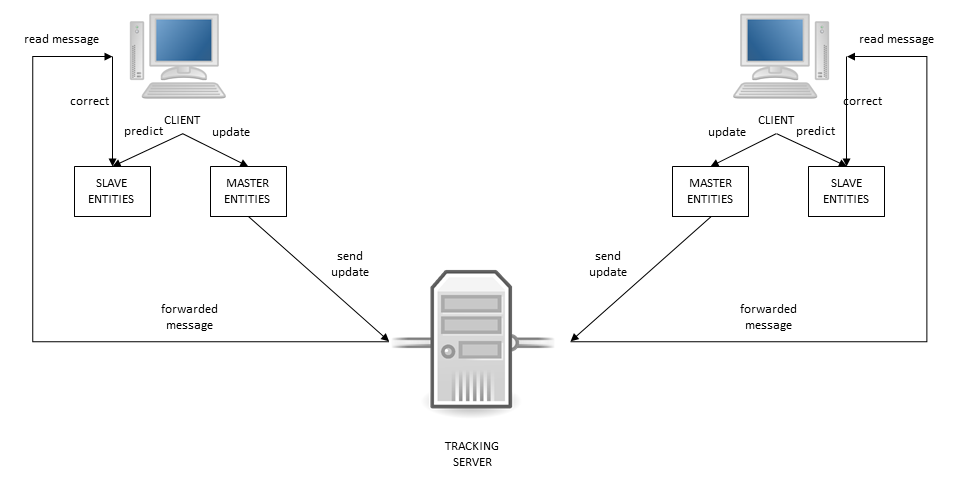
\includegraphics[scale=0.3]{Figures/masterslave}
	\caption{Master/slave architecture}
	\label{fig:masterslave}
\end{figure}